\chapter{Structure}


Dans ce chapitre nous présentons des explications générales sur le positionnement du corps.
Nous donnons aussi des exercices pour aider à prendre conscience des positions et des sensations ainsi qu'à construire certains automatismes.
La position de garde est aussi discutée.


%%%%%%%%%%%%%%%%%%%%%%%%%%%%%%%%%%%%%%
\section{L'importance de la structure}
%%%%%%%%%%%%%%%%%%%%%%%%%%%%%%%%%%%%%%
\label{sec:structure:général}


La structure du corps est un élément clé de l'escrime : bien plus que la technique la structure détermine comment on va réagir à une attaque adverse.
Porter une attaque en escrime ne se réduit pas à un simple mouvement du bras : pour que le coup soit efficace il faut que tout le corps contribue à l'action.
Un coup qui est porté seulement avec le bras paraîtra mécanique et peu naturel, tandis qu'une action sollicitant tout le corps sera fluide et harmonieuse.
Il sera plus compliqué de résister avec une structure faible, même contre une attaque mal exécutée.
De plus il est aussi plus difficile de réaliser correctement les techniques.
Enfin une mauvaise position du corps entraîne des tensions inutiles qui peuvent accroître le risque de blessures et contribuer à l'apparition de douleurs sur le long terme (tendinite, douleur au genou…).
Pour ces différentes raisons il est important de prêter dès que possible attention à la position du corps et de garder cette question toujours en tête, même après plusieurs années de pratique.

Il peut être frustrant de chercher à améliorer la position du corps car c'est quelque chose qui prend énormément de temps : nous avons été habitués pendant des années à avoir une certaine position (souvent mauvaise), et là il faut en apprendre une autre, qui paraît souvent moins naturelle.
Une première étape est d'apprendre à écouter les sensations du corps : l'escrime est logique et efficace, et de ce fait l'on n'est pas censé être mal à l'aise dans une position.
Ainsi si l'on ressent une gêne quelconque en effectuant une technique ou en prenant une certaine position alors cela signifie que l'on a un problème de structure (ou bien que l'on a mal compris la position demandée).
Il peut être utile, régulièrement, de s'arrêter -- par exemple à la fin d'une technique ou même d'un coup (en ayant prévenu son partenaire) -- afin de tourner son attention vers son corps.

Il peut être intéressant de travailler sans gants (en prenant les précautions nécessaires) pour vraiment sentir la poignée et le sentiment de la lame~\cite{enzi:dijon:messer_inner:2015}.
Idem travailler sans chaussures permet de mieux sentir le sol (historiquement on se battait sans chaussures ou avec des semelles de \SI{1}{mm}).


\section{Position de garde}


La position de garde est la position que le corps adopte lors de l'attente et entre chaque attaque.
Il s'agit d'une position robuste, qui permet d'absorber les coups, et dynamique, qui permet de réagir rapidement (aussi bien en attaque qu'en défense) tout en améliorant l'efficacité des mouvements.
Le "côté" d'une garde est défini par le pied qui se trouve à l'avant.


\begin{definition}[Position de garde standard]
\label{struc:def:position-garde}

La position de garde est la suivante :
\begin{itemize}
	\item les genoux sont déverrouillés et les jambes fléchies ;
	\item le pied arrière est tourné de \ang{45} sur le côté (parfois jusqu'à 90°), le pied avant est pointé droit devant (figure~\ref{struc:fig:garde-pieds}) ;
	\item les deux pieds sont séparés une ligne ;
	\item les coudes ne sont jamais tendus ;
	\item le dos est droit, le buste est tourné à \ang{45} ;
	\item le bassin est basculé vers l'avant ;
	\item les épaules sont décontractées.
	% gainage éventuel
\end{itemize}
\end{definition}


\begin{figure}[ht]
	\centering
	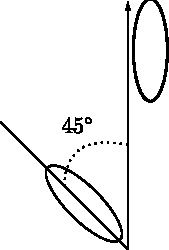
\includegraphics[scale=1]{structure/garde_pieds.pdf}
	\caption{Position des pieds pour la garde standard de la définition~\ref{struc:def:position-garde}.
	Le pied avant est pointé vers l'opposant, le pied arrière à \ang{45}, avec un léger écart entre les deux.
	La distance entre les deux talons est égale à la largeur des épaules.}
	\label{struc:fig:garde-pieds}
\end{figure}


\noindent
Expliquons maintenant certains des points précédents :
\begin{itemize}
	\item jambes fléchies : cela permet d'abaisser le centre de gravité et d'être plus stable, et ainsi de mieux résister en cas de chocs ou de poussée (le pire étant d'avoir les jambes totalement tendues) ;
	
	\item pied avant vers l'adversaire : l'alignement du pied définit la direction d'attaque et d'avancée : ainsi si le pied pointe sur le côté, une marche entraînera du mauvais côté ;
	
	\item coudes fléchis : des coudes tendus offrent une bonne cible pour placer une clé au corps-à-corps, augmentent le risque de se faire mal aux articulations (à force de buter) et enfin diminuent la rapidité de mouvement ;
	
	\item buste de profil : cela permet d'offrir une cible plus réduite à l'opposant tout en augmentant la portée de l'arme tenue dans la main avant.
\end{itemize}
Les deux premiers éléments sont certainement parmi les plus importants.
Le lecteur est encouragé à expérimenter et à se convaincre que la position de garde proposée est celle qui propose une stabilité maximale (exercice~\ref{struc:ex:test-position} ci-dessous).

Le stabilité est importante si l'adversaire cherche à pousser ou à tirer.
De même les mouvements (pour revenir en garde, se déplacer, attaquer) seront plus rapides si les jambes sont fléchis.
Finalement la force de la frappe est augmentée si l'on peut mobiliser tout le corps, ce qui est facilité par la position décrite ci-dessus.

\begin{exercice}

\begin{enumerate}
	\item \A porte une attaque dans le vide et s'arrête.
	
	\item \D attrape la main de \A et tirer pour vérifier s'il est stable.
\end{enumerate}
\end{exercice}

Il faut noter que la position décrite dans cette section correspond à celle utilisée avec de nombreuses armes, mais il ne s'agit pas de la seule.
Par exemple le buste est penché vers l'avant dans la garde à l'épée-bocle (style I.33), tandis que le buste est beaucoup plus de profil à la rapière ou encore le second pied peut se trouver presque vers l'avant en combat rapproché.
Nous introduirons les gardes adaptées aux différentes armes dans les chapitres traitant de celles-ci.

% Thomas
Un bon repère est d'avoir le genou au-dessus du pied, afin que le mollet soit bien vertical, tandis que la cuisse est dans l'axe du pied.
De plus la distance entre les deux talons est égale à la largeur des épaules.
Cela permet de préserver les genoux et d'être plus stable.

Il n'est pas toujours facile au début de trouver la bonne position.
Le fait de se sentir à l'aise est un critère important.
Nous proposons deux exercices qui permettent d'adopter facilement une garde correcte.


\begin{exercice}[Trouver la position des pieds]

Marcher naturellement et s'arrêter (pied droit devant).

Au moment de s'arrêter les pieds se trouvent naturellement dans une position de garde.
Il ne reste plus qu'à se baisser sur ses appuis.

\source{\cite{guidoux:dijon:thibault:2015}.}

\end{exercice}


\begin{exercice}[Trouver une bonne garde]

Se tenir pied joint, sauter en l'air et retomber jambes écartées (droite devant, gauche en arrière).

\source{\cite{enzi:dijon:messer_inner:2015}.}

\end{exercice}


\begin{exercice}[Comparaison de positions faible et forte]
\label{struc:ex:test-position}

\obj{Sentir quels éléments de la position permettent à \D de résister plus facilement à la poussée de \A.}

\A et \D travaillent ensemble.
\D adopte une certaine position de garde, puis \A pose ses mains sur \D (épaule ou poitrine) et essaie de pousser.
\D peut essayer de résister.
La position adoptée par \D est variée entre les deux extrêmes :
\begin{enumerate}
	\item \D se tient debout, jambes tendues et de face.
	\item \D adopte la garde de la définition~\ref{struc:def:position-garde}.
\end{enumerate}

Il n'est pas nécessaire d'y aller fort et de faire mal au partenaire : l'intérêt est plutôt de voir comment \D réagit à une poussée constante.

\end{exercice}


Lorsque deux adversaires se font face les axes définis par les pieds avant sont alignés (figure~\ref{struc:fig:garde-pieds-duel}).

\begin{figure}[ht]
	\centering
	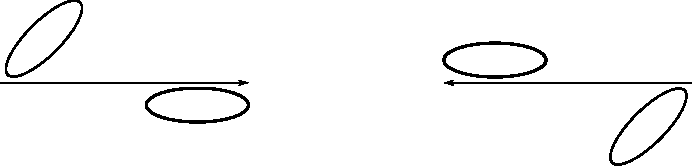
\includegraphics[scale=1]{structure/garde_pieds_duel.pdf}
	\caption{Position des pieds pour la garde standard de la définition~\ref{struc:def:position-garde}.
	L'axe des deux adversaires est aligné.}
	\label{struc:fig:garde-pieds-duel}
\end{figure}


\begin{exercice}[L'échauffement d'Ingulf]
\label{struc:ex:Ingulf}
\index{echauffement@échauffement!exercice}

\obj{Cet exercice travaille la structure et l'équilibre.}

\begin{enumerate}
	\item \A et \D sont en position de garde, pied droit devant.
	De la main droite \A saisit l'intérieur du coude gauche de \D, tandis que de la main gauche il saisit l'extérieur du bras droit (haut de l'avant-bras/coude).
	\D fait de même : la position est totalement symétrique entre \A et \D.
	
	\item \A et \D se déplacent en essayant de diriger les mouvements de l'autre et en testant son équilibre.
\end{enumerate}

L'objectif de l'exercice est de ressentir ce qui se passe et d'utiliser les mouvements du partenaire pour le déséquilibrer et l'emmener dans la direction que l'on souhaite.
Ainsi ce travail privilégie la sensation et non la force brute : pousser comme un barbare et serrant fort son partenaire n'a aucun intérêt.
Voici quelques pistes pour tirer parti de cet exercice :
\begin{itemize}
	\item Comparer la difficulté de résister en fonction de la position adoptée (que ce soit par soi-même ou par son partenaire).
	
	\item Sentir que si \A pousse dans une direction alors \D peut le déséquilibrer et augmenter l'amplitude du mouvement de \A en se dérobant et en le tirant dans la direction d'origine.
	Cela est d'autant plus efficace contre quelqu'un qui utilise la force brute.
\end{itemize}

Des variantes à cet exercice qui permettent de travailler le sentiment du contact sont données dans l'exercice~\ref{att:ex:Ingulf-variantes}.

\source{\cite{Kohlweiss:2014:Dijon:RingenSchwert}}

\end{exercice}


\section{Hanches}


Ainsi que nous l'avons vu plus haut, un défaut important du débutant (et qui peut perdurer longtemps) est de dissocier les différentes parties du corps.
On a souvent tendance à utiliser uniquement les bras et les épaules pour les mouvements, alors qu'un mouvement efficace mobilise le corps entier.
Les hanches sont très importantes pour unifier tout le corps, et les mouvements devraient partir de celles-ci en priorité.


\begin{exercice}
En position de garde, se pencher en avant et laisser le bras ballant du côté de la jambe arrière (type lancer de pétanque).
Grâce à un mouvement de hanches laisser le bras se balancer d'avant en arrière, puis de plus en plus vite jusqu'à faire des cercles.

\source{\cite{enzi:dijon:messer_inner:2015}}
\end{exercice}


\begin{exercice}[La roue (en avant)]
\label{struc:ex:roue-avant}

\obj{La position du corps fait qu'il est nécessaire de mobiliser les hanches lors du mouvement.}

Dans la description de cet exercice nous donnons d'abord la position de départ, puis le mouvement qui permet d'effectuer la transition vers la position suivante, elle-même décrite dans un point séparé.
Cette position sert alors de départ pour la transition suivante, et ainsi de suite : cet exercice est cyclique et peut être travaillé en faisant des longueurs dans le gymnase.

\begin{enumerate}
	\item Position verticale : de face, talons joints, léger angle entre les pieds, bras tendus parallèles au corps (le gauche vers le haut, le droit vers le bas).
	
	\item Transition : avancer le pied droit en levant le bras droit vers l'avant et en basculant le bras gauche vers l'arrière.
	
	\item Position horizontale : de profil, position de profil, pieds en position de garde (jambe droite en avant), bras tendus parallèles au sol (le droit vers l'avant, le gauche vers l'arrière).
	
	\item Transition : avancer le pied gauche à côté du pied droit, le bras gauche bascule vers le bas, le bras droit se lève vers le haut.
	
	\item Position verticale (symétrique par rapport à 1.).
\end{enumerate}

Pendant tous l'enchaînement (en particulier dans la position verticale) les genoux sont légèrement pliés.
Chaque partir du corps reste à la même hauteur : en particulier la tête et les épaules tracent une ligne parallèle au sol (i.e.\ le corps ne fait pas une vague en bougeant -- on retrouve cette idée dans la valse).

Après une certaine pratique on pourra chercher à effectuer la transition dynamiquement, avec l'idée que l'on est en train d'attaquer vers l'avant.

% Jean-Paul
\source{Échauffement en Katori Shinto Ryu.}
\end{exercice}


\begin{exercice}[La roue (en arrière)]
\label{struc:ex:roue-arrière}

\begin{enumerate}
	\item Position verticale : de face, talons joints, léger angle entre les pieds, bras tendus parallèles au corps (le gauche vers le haut, le droit vers le bas).
	
	\item Transition : reculer le pied gauche en levant le bras droit vers l'avant et en basculant le bras gauche vers l'arrière.
	
	\item Position horizontale : de profil, position de profil, pieds en position de garde (jambe droite en avant), bras tendus parallèles au sol (le droit vers l'avant, le gauche vers l'arrière).
	
	\item Transition : avancer le pied gauche à côté du pied droit, le bras gauche bascule vers le bas, le bras droit se lève vers le haut.
	
	\item Position verticale (symétrique par rapport à 1.).
\end{enumerate}

La différence avec le mouvement principale est que l'on recule le pied gauche lors du premier mouvement.
Toutefois la position horizontale est la même que dans l'exercice précédent.

% Jean-Paul
\source{Échauffement en Katori Shinto Ryu.}
\end{exercice}


% TODO: déplacer ailleurs
\begin{exercice}[La roue (à deux)]
\label{struc:ex:roue-deux}

% on y reviendra
\obj{Cet exercice permet de prendre conscience de l'occupation du centre de la ligne ainsi que de s'entraîner à agir en même temps que son partenaire.}

\A et \D se font face.
\A et \D exécutent respectivement une roue vers l'avant et une roue vers l'arrière, en simultané.

Du fait que seul le mouvement des pieds est inversé \A et \D terminent dans une position symétrique, avec leurs bras parallèles.
La distance entre \A et \D est de telle sorte que, en position horizontale, la main se situe au niveau de la poitrine du partenaire (sans le mouvement, le buste serait touché, l'esquive se fait parce que l'on se retrouve de profil).

% Jean-Paul
\source{Échauffement en Katori Shinto Ryu.}
\end{exercice}


\begin{exercice}

\obj{Sentir que le mouvement des hanches est nécessaire pour enchaîner efficacement les quatre frappes.}

\A travaille seul avec une arme quelconque~\footnotemark{}.
\footnotetext{À ce stade les attaques et défenses n'ont pas été abordées.
Pour cette raison le lecteur pourra ignorer cet exercice dans un premier.}

\begin{enumerate}
	\item Départ en position de garde à gauche, pied droit devant.
	
	\item En avançant le pied gauche, monter l'épée en garde haute à gauche puis frappe à gauche à la tête.
	Léger retour en garde.
	
	\item Avancer le pied droit en attaquant en face ou à droite, retour en garde à gauche.
	
	\item Faire un demi-tour en passant le pied droit derrière, en tournant autour du côté de gauche (le talon gauche sert de point de pivot), en frappant par en dessous (l'épée est presque dans un plan perpendiculaire au sol).
	
	\item Faire un demi-tour en passant le pied droit derrière, en tournant autour du côté de gauche (le talon gauche sert de point de pivot), en frappant à droite.
\end{enumerate}
Cet exercice peut aussi être pratiqué en reculant : les mêmes frappes sont effectuées, mais le mouvement des jambes est inversé.

La précision des attaques n'est pas importante au début, il vaut mieux se concentrer sur la rotation des hanches.
Dans un second temps on pourra s'assurer que les gardes et attaques ont un sens.

Les attaques et défenses précises doivent être adaptées en fonction de l'arme considérée.
Voici quelques exemples :
\begin{itemize}
	\item épée longue : 1) charrue à gauche, 2) frappe à gauche du vrai tranchant (donc en décroisant les mains) à partir d'un bœuf à gauche, 3) estoc, 4) unterhau à droite, 5) oberhau à droite ;
	
	\item mains nues : 2) direct gauche, 3) direct droit, 4) uppercut droit, 5) frappe descendante avec le talon du poing droit ;
	
	\item close combat : 2) tranche de la main droite en descendant (en revers), 3) percussion avec le talon de la paume droite, 4) percussion avec le talon de la paume droite, 5) tranche de la main droite en descendant.
	
% 	\item rapière : 1) quarte, 2) estoc puis tierce, 3) taille puis quarte, 4) estoc, 5) taille.
	
	% bokken : 1) garde de face, 2) idem que épée longue, 3) maki-uchi, 4) idem, 5) attaque via jodan
\end{itemize}

Il peut être intéressant de répéter l'exercice et d'avoir quelqu'un qui donne le signal pour donner un certain rythme.

% Jean-Paul
\source{Échauffement en Katori Shinto Ryu.}
\end{exercice}


\section{Respiration}


Dans un premier lieu il faut savoir gérer sa respiration afin de ne pas se retrouver à court de souffle, surtout lors du combat libre et lorsqu'il fait chaud (et ce d'autant plus lorsque l'on porte un masque ou d'autres protections).
De plus le souffle permet de rythmer efficacement les mouvements, et en particulier les frappes, en expirant au moment de porter le coup.
Cette dernière idée a été particulièrement développée dans l'escrime japonaise où (presque) chaque coup est accompagnée d'un kiai.


\begin{exercice}[Frapper en expirant]

Choisir une frappe et s'entraîner à expirer en portant le coup.

\end{exercice}


\section{Résumé}


Dans ce chapitre nous avons vu que disposer d'une bonne structure est important.
En particulier les points suivants donnent des éléments pour améliorer la structure :
\begin{itemize}
	\item avoir une bonne position de garde : jambes fléchies, pied arrière à 45°, pied avant vers le partenaire, dos droit, bassin basculé ;
	\item faire attention au rôle des hanches afin d'unifier le corps ;
	\item expirer en frappant.
\end{itemize}


